\documentclass[1p]{elsarticle_modified}
%\bibliographystyle{elsarticle-num}

%\usepackage[colorlinks]{hyperref}
%\usepackage{abbrmath_seonhwa} %\Abb, \Ascr, \Acal ,\Abf, \Afrak
\usepackage{amsfonts}
\usepackage{amssymb}
\usepackage{amsmath}
\usepackage{amsthm}
\usepackage{scalefnt}
\usepackage{amsbsy}
\usepackage{kotex}
\usepackage{caption}
\usepackage{subfig}
\usepackage{color}
\usepackage{graphicx}
\usepackage{xcolor} %% white, black, red, green, blue, cyan, magenta, yellow
\usepackage{float}
\usepackage{setspace}
\usepackage{hyperref}

\usepackage{tikz}
\usetikzlibrary{arrows}

\usepackage{multirow}
\usepackage{array} % fixed length table
\usepackage{hhline}

%%%%%%%%%%%%%%%%%%%%%
\makeatletter
\renewcommand*\env@matrix[1][\arraystretch]{%
	\edef\arraystretch{#1}%
	\hskip -\arraycolsep
	\let\@ifnextchar\new@ifnextchar
	\array{*\c@MaxMatrixCols c}}
\makeatother %https://tex.stackexchange.com/questions/14071/how-can-i-increase-the-line-spacing-in-a-matrix
%%%%%%%%%%%%%%%

\usepackage[normalem]{ulem}

\newcommand{\msout}[1]{\ifmmode\text{\sout{\ensuremath{#1}}}\else\sout{#1}\fi}
%SOURCE: \msout is \stkout macro in https://tex.stackexchange.com/questions/20609/strikeout-in-math-mode

\newcommand{\cancel}[1]{
	\ifmmode
	{\color{red}\msout{#1}}
	\else
	{\color{red}\sout{#1}}
	\fi
}

\newcommand{\add}[1]{
	{\color{blue}\uwave{#1}}
}

\newcommand{\replace}[2]{
	\ifmmode
	{\color{red}\msout{#1}}{\color{blue}\uwave{#2}}
	\else
	{\color{red}\sout{#1}}{\color{blue}\uwave{#2}}
	\fi
}

\newcommand{\Sol}{\mathcal{S}} %segment
\newcommand{\D}{D} %diagram
\newcommand{\A}{\mathcal{A}} %arc


%%%%%%%%%%%%%%%%%%%%%%%%%%%%%5 test

\def\sl{\operatorname{\textup{SL}}(2,\Cbb)}
\def\psl{\operatorname{\textup{PSL}}(2,\Cbb)}
\def\quan{\mkern 1mu \triangleright \mkern 1mu}

\theoremstyle{definition}
\newtheorem{thm}{Theorem}[section]
\newtheorem{prop}[thm]{Proposition}
\newtheorem{lem}[thm]{Lemma}
\newtheorem{ques}[thm]{Question}
\newtheorem{cor}[thm]{Corollary}
\newtheorem{defn}[thm]{Definition}
\newtheorem{exam}[thm]{Example}
\newtheorem{rmk}[thm]{Remark}
\newtheorem{alg}[thm]{Algorithm}

\newcommand{\I}{\sqrt{-1}}
\begin{document}

%\begin{frontmatter}
%
%\title{Boundary parabolic representations of knots up to 8 crossings}
%
%%% Group authors per affiliation:
%\author{Yunhi Cho} 
%\address{Department of Mathematics, University of Seoul, Seoul, Korea}
%\ead{yhcho@uos.ac.kr}
%
%
%\author{Seonhwa Kim} %\fnref{s_kim}}
%\address{Center for Geometry and Physics, Institute for Basic Science, Pohang, 37673, Korea}
%\ead{ryeona17@ibs.re.kr}
%
%\author{Hyuk Kim}
%\address{Department of Mathematical Sciences, Seoul National University, Seoul 08826, Korea}
%\ead{hyukkim@snu.ac.kr}
%
%\author{Seokbeom Yoon}
%\address{Department of Mathematical Sciences, Seoul National University, Seoul, 08826,  Korea}
%\ead{sbyoon15@snu.ac.kr}
%
%\begin{abstract}
%We find all boundary parabolic representation of knots up to 8 crossings.
%
%\end{abstract}
%\begin{keyword}
%    \MSC[2010] 57M25 
%\end{keyword}
%
%\end{frontmatter}

%\linenumbers
%\tableofcontents
%
\newcommand\colored[1]{\textcolor{white}{\rule[-0.35ex]{0.8em}{1.4ex}}\kern-0.8em\color{red} #1}%
%\newcommand\colored[1]{\textcolor{white}{ #1}\kern-2.17ex	\textcolor{white}{ #1}\kern-1.81ex	\textcolor{white}{ #1}\kern-2.15ex\color{red}#1	}

{\Large $\underline{11a_{5}~(K11a_{5})}$}

\setlength{\tabcolsep}{10pt}
\renewcommand{\arraystretch}{1.6}
\vspace{1cm}\begin{tabular}{m{100pt}>{\centering\arraybackslash}m{274pt}}
\multirow{5}{120pt}{
	\centering
	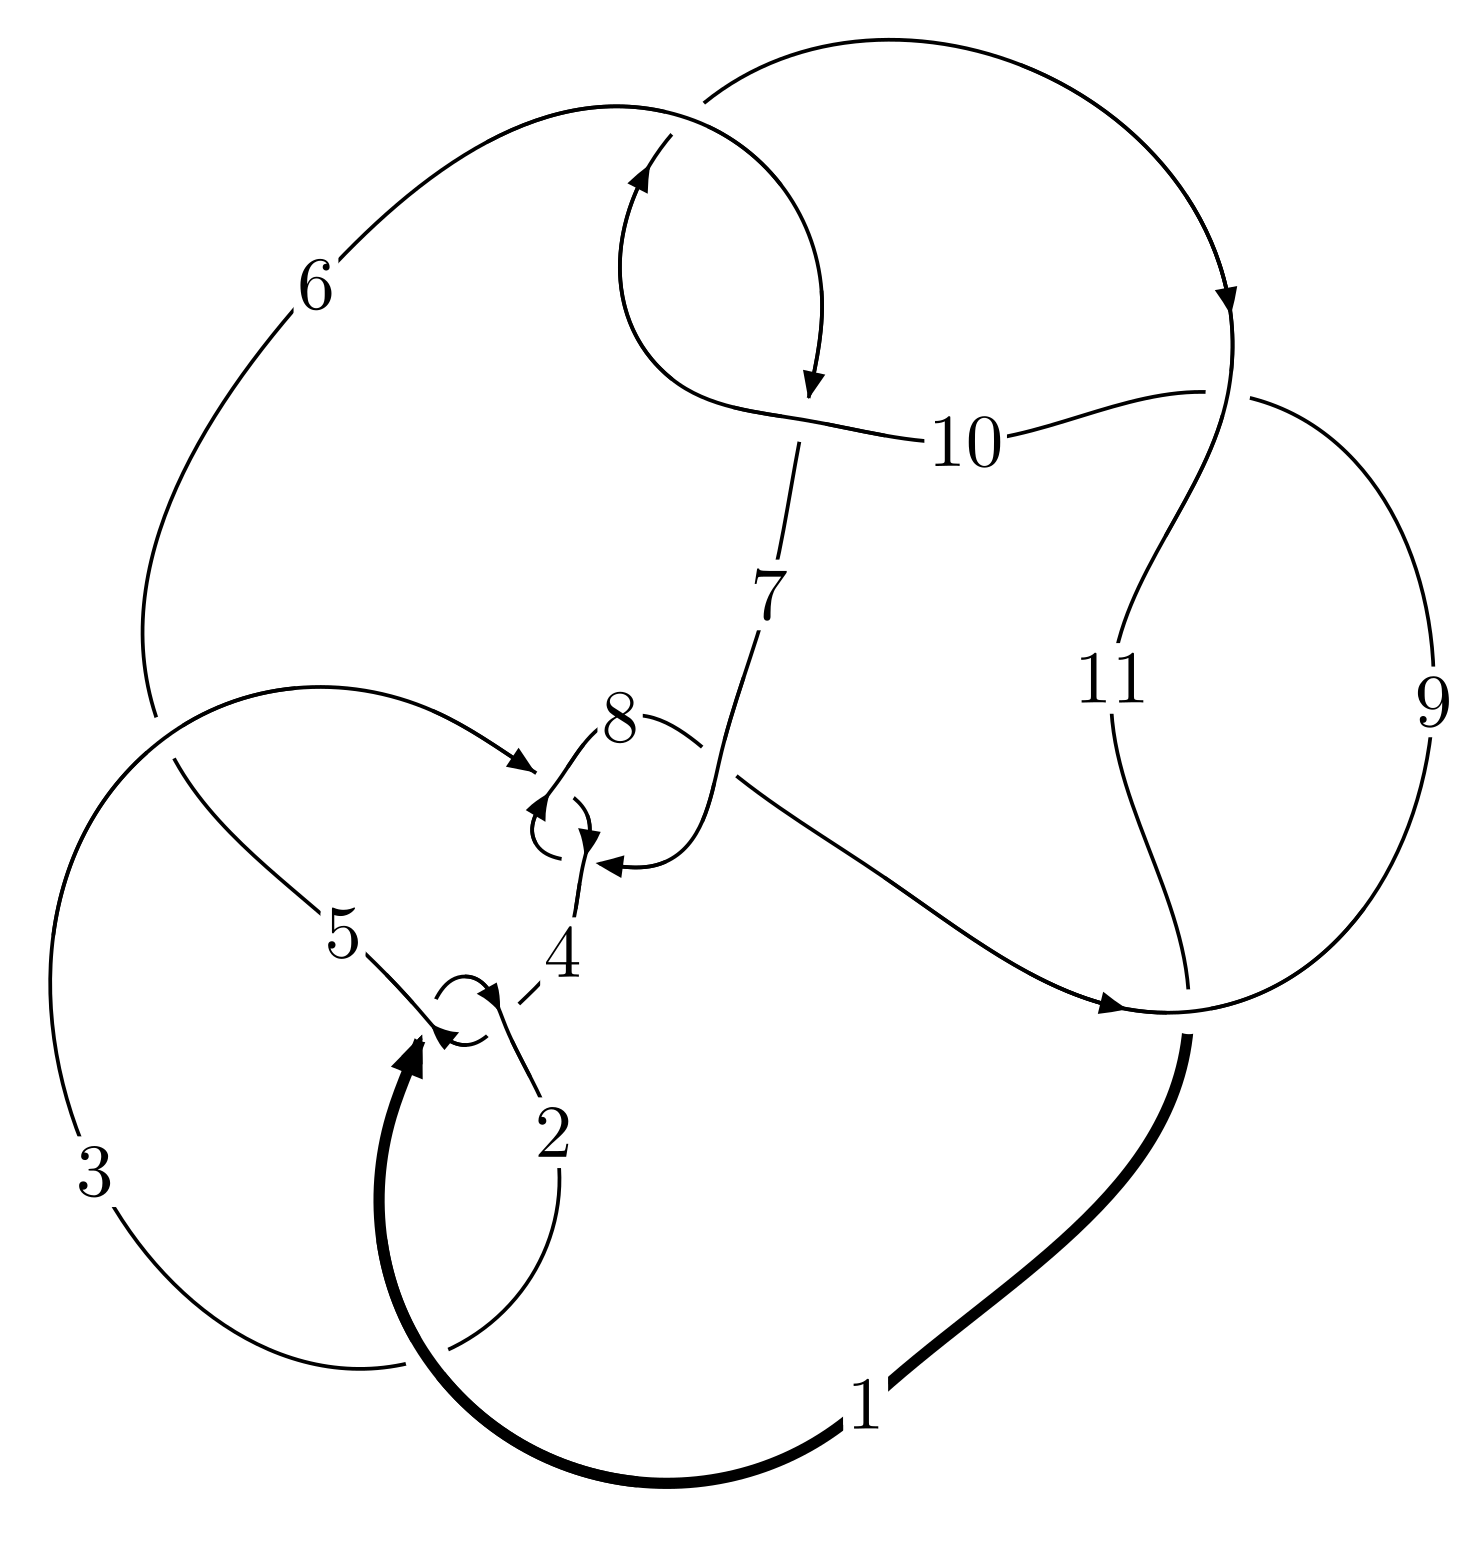
\includegraphics[width=112pt]{../../../GIT/diagram.site/Diagrams/png/254_11a_5.png}\\
\ \ \ A knot diagram\footnotemark}&
\allowdisplaybreaks
\textbf{Linearized knot diagam} \\
\cline{2-2}
 &
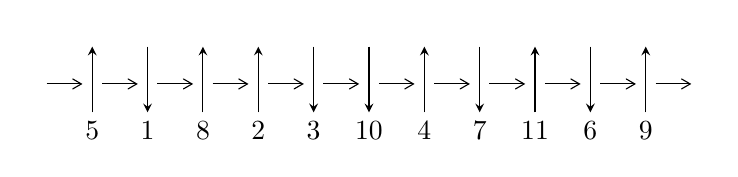
\begin{tikzpicture}[x=20pt, y=17pt]
	% nodes
	\node (C0) at (0, 0) {};
	\node (C1) at (1, 0) {};
	\node (C1U) at (1, +1) {};
	\node (C1D) at (1, -1) {5};

	\node (C2) at (2, 0) {};
	\node (C2U) at (2, +1) {};
	\node (C2D) at (2, -1) {1};

	\node (C3) at (3, 0) {};
	\node (C3U) at (3, +1) {};
	\node (C3D) at (3, -1) {8};

	\node (C4) at (4, 0) {};
	\node (C4U) at (4, +1) {};
	\node (C4D) at (4, -1) {2};

	\node (C5) at (5, 0) {};
	\node (C5U) at (5, +1) {};
	\node (C5D) at (5, -1) {3};

	\node (C6) at (6, 0) {};
	\node (C6U) at (6, +1) {};
	\node (C6D) at (6, -1) {10};

	\node (C7) at (7, 0) {};
	\node (C7U) at (7, +1) {};
	\node (C7D) at (7, -1) {4};

	\node (C8) at (8, 0) {};
	\node (C8U) at (8, +1) {};
	\node (C8D) at (8, -1) {7};

	\node (C9) at (9, 0) {};
	\node (C9U) at (9, +1) {};
	\node (C9D) at (9, -1) {11};

	\node (C10) at (10, 0) {};
	\node (C10U) at (10, +1) {};
	\node (C10D) at (10, -1) {6};

	\node (C11) at (11, 0) {};
	\node (C11U) at (11, +1) {};
	\node (C11D) at (11, -1) {9};
	\node (C12) at (12, 0) {};

	% arrows
	\draw[->,>={angle 60}]
	(C0) edge (C1) (C1) edge (C2) (C2) edge (C3) (C3) edge (C4) (C4) edge (C5) (C5) edge (C6) (C6) edge (C7) (C7) edge (C8) (C8) edge (C9) (C9) edge (C10) (C10) edge (C11) (C11) edge (C12) ;	\draw[->,>=stealth]
	(C1D) edge (C1U) (C2U) edge (C2D) (C3D) edge (C3U) (C4D) edge (C4U) (C5U) edge (C5D) (C6U) edge (C6D) (C7D) edge (C7U) (C8U) edge (C8D) (C9D) edge (C9U) (C10U) edge (C10D) (C11D) edge (C11U) ;
	\end{tikzpicture} \\
\hhline{~~} \\& 
\textbf{Solving Sequence} \\ \cline{2-2} 
 &
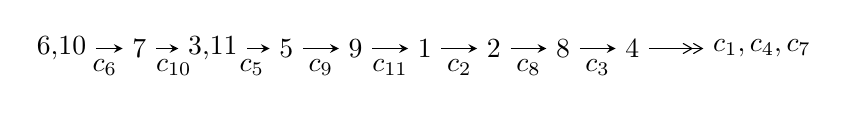
\begin{tikzpicture}[x=25pt, y=7pt]
	% node
	\node (A0) at (-1/8, 0) {6,10};
	\node (A1) at (1, 0) {7};
	\node (A2) at (33/16, 0) {3,11};
	\node (A3) at (25/8, 0) {5};
	\node (A4) at (33/8, 0) {9};
	\node (A5) at (41/8, 0) {1};
	\node (A6) at (49/8, 0) {2};
	\node (A7) at (57/8, 0) {8};
	\node (A8) at (65/8, 0) {4};
	\node (C1) at (1/2, -1) {$c_{6}$};
	\node (C2) at (3/2, -1) {$c_{10}$};
	\node (C3) at (21/8, -1) {$c_{5}$};
	\node (C4) at (29/8, -1) {$c_{9}$};
	\node (C5) at (37/8, -1) {$c_{11}$};
	\node (C6) at (45/8, -1) {$c_{2}$};
	\node (C7) at (53/8, -1) {$c_{8}$};
	\node (C8) at (61/8, -1) {$c_{3}$};
	\node (A9) at (10, 0) {$c_{1},c_{4},c_{7}$};

	% edge
	\draw[->,>=stealth]	
	(A0) edge (A1) (A1) edge (A2) (A2) edge (A3) (A3) edge (A4) (A4) edge (A5) (A5) edge (A6) (A6) edge (A7) (A7) edge (A8) ;
	\draw[->>,>={angle 60}]	
	(A8) edge (A9);
\end{tikzpicture} \\ 

\end{tabular} \\

\footnotetext{
The image of knot diagram is generated by the software ``\textbf{Draw programme}" developed by Andrew Bartholomew(\url{http://www.layer8.co.uk/maths/draw/index.htm\#Running-draw}), where we modified some parts for our purpose(\url{https://github.com/CATsTAILs/LinksPainter}).
}\phantom \\ \newline 
\centering \textbf{Ideals for irreducible components\footnotemark of $X_{\text{par}}$} 
 
\begin{align*}
I^u_{1}&=\langle 
u^{55}+2 u^{54}+\cdots+2 b-2,\;-3 u^{55}-9 u^{54}+\cdots+2 a-1,\;u^{56}+3 u^{55}+\cdots+2 u+1\rangle \\
I^u_{2}&=\langle 
b+u,\;a- u+1,\;u^2- u+1\rangle \\
I^u_{3}&=\langle 
- u^3+b- u,\;u^3+a,\;u^{10}+2 u^8+3 u^6- u^5+2 u^4- u^3+u^2- u+1\rangle \\
I^u_{4}&=\langle 
b- u+1,\;a-1,\;u^2- u+1\rangle \\
\\
\end{align*}
\raggedright * 4 irreducible components of $\dim_{\mathbb{C}}=0$, with total 70 representations.\\
\footnotetext{All coefficients of polynomials are rational numbers. But the coefficients are sometimes approximated in decimal forms when there is not enough margin.}
\newpage
\renewcommand{\arraystretch}{1}
\centering \section*{I. $I^u_{1}= \langle u^{55}+2 u^{54}+\cdots+2 b-2,\;-3 u^{55}-9 u^{54}+\cdots+2 a-1,\;u^{56}+3 u^{55}+\cdots+2 u+1 \rangle$}
\flushleft \textbf{(i) Arc colorings}\\
\begin{tabular}{m{7pt} m{180pt} m{7pt} m{180pt} }
\flushright $a_{6}=$&$\begin{pmatrix}1\\0\end{pmatrix}$ \\
\flushright $a_{10}=$&$\begin{pmatrix}0\\u\end{pmatrix}$ \\
\flushright $a_{7}=$&$\begin{pmatrix}1\\u^2\end{pmatrix}$ \\
\flushright $a_{3}=$&$\begin{pmatrix}\frac{3}{2} u^{55}+\frac{9}{2} u^{54}+\cdots+3 u+\frac{1}{2}\\-\frac{1}{2} u^{55}- u^{54}+\cdots+\frac{1}{2} u+1\end{pmatrix}$ \\
\flushright $a_{11}=$&$\begin{pmatrix}- u\\u\end{pmatrix}$ \\
\flushright $a_{5}=$&$\begin{pmatrix}-\frac{1}{2} u^{55}-\frac{3}{2} u^{54}+\cdots+2 u-\frac{1}{2}\\\frac{1}{2} u^{55}+u^{54}+\cdots-\frac{7}{2} u^2+\frac{3}{2} u\end{pmatrix}$ \\
\flushright $a_{9}=$&$\begin{pmatrix}- u^3\\u^3+u\end{pmatrix}$ \\
\flushright $a_{1}=$&$\begin{pmatrix}- u^5- u\\u^5+u^3+u\end{pmatrix}$ \\
\flushright $a_{2}=$&$\begin{pmatrix}u^{55}+\frac{3}{2} u^{54}+\cdots+\frac{1}{2} u-\frac{1}{2}\\\frac{3}{2} u^{55}+5 u^{54}+\cdots+\frac{9}{2} u+3\end{pmatrix}$ \\
\flushright $a_{8}=$&$\begin{pmatrix}u^5+u\\u^7+u^5+2 u^3+u\end{pmatrix}$ \\
\flushright $a_{4}=$&$\begin{pmatrix}\frac{3}{2} u^{55}+\frac{13}{2} u^{54}+\cdots+4 u+\frac{3}{2}\\-\frac{3}{2} u^{55}-5 u^{54}+\cdots-\frac{3}{2} u-1\end{pmatrix}$\\ \flushright $a_{4}=$&$\begin{pmatrix}\frac{3}{2} u^{55}+\frac{13}{2} u^{54}+\cdots+4 u+\frac{3}{2}\\-\frac{3}{2} u^{55}-5 u^{54}+\cdots-\frac{3}{2} u-1\end{pmatrix}$\\&\end{tabular}
\flushleft \textbf{(ii) Obstruction class $= -1$}\\~\\
\flushleft \textbf{(iii) Cusp Shapes $= \frac{3}{2} u^{55}+6 u^{54}+\cdots+\frac{21}{2} u+10$}\\~\\
\newpage\renewcommand{\arraystretch}{1}
\flushleft \textbf{(iv) u-Polynomials at the component}\newline \\
\begin{tabular}{m{50pt}|m{274pt}}
Crossings & \hspace{64pt}u-Polynomials at each crossing \\
\hline $$\begin{aligned}c_{1},c_{4}\end{aligned}$$&$\begin{aligned}
&u^{56}+3 u^{55}+\cdots+4 u+1
\end{aligned}$\\
\hline $$\begin{aligned}c_{2}\end{aligned}$$&$\begin{aligned}
&u^{56}+27 u^{55}+\cdots+12 u+1
\end{aligned}$\\
\hline $$\begin{aligned}c_{3},c_{7}\end{aligned}$$&$\begin{aligned}
&u^{56}+4 u^{55}+\cdots+48 u+16
\end{aligned}$\\
\hline $$\begin{aligned}c_{5}\end{aligned}$$&$\begin{aligned}
&u^{56}-3 u^{55}+\cdots-228 u+73
\end{aligned}$\\
\hline $$\begin{aligned}c_{6},c_{10}\end{aligned}$$&$\begin{aligned}
&u^{56}-3 u^{55}+\cdots-2 u+1
\end{aligned}$\\
\hline $$\begin{aligned}c_{8}\end{aligned}$$&$\begin{aligned}
&u^{56}+20 u^{55}+\cdots+1920 u+256
\end{aligned}$\\
\hline $$\begin{aligned}c_{9},c_{11}\end{aligned}$$&$\begin{aligned}
&u^{56}-19 u^{55}+\cdots-12 u+1
\end{aligned}$\\
\hline
\end{tabular}\\~\\
\newpage\renewcommand{\arraystretch}{1}
\flushleft \textbf{(v) Riley Polynomials at the component}\newline \\
\begin{tabular}{m{50pt}|m{274pt}}
Crossings & \hspace{64pt}Riley Polynomials at each crossing \\
\hline $$\begin{aligned}c_{1},c_{4}\end{aligned}$$&$\begin{aligned}
&y^{56}+27 y^{55}+\cdots+12 y+1
\end{aligned}$\\
\hline $$\begin{aligned}c_{2}\end{aligned}$$&$\begin{aligned}
&y^{56}+7 y^{55}+\cdots+20 y+1
\end{aligned}$\\
\hline $$\begin{aligned}c_{3},c_{7}\end{aligned}$$&$\begin{aligned}
&y^{56}+20 y^{55}+\cdots+1920 y+256
\end{aligned}$\\
\hline $$\begin{aligned}c_{5}\end{aligned}$$&$\begin{aligned}
&y^{56}-13 y^{55}+\cdots-28332 y+5329
\end{aligned}$\\
\hline $$\begin{aligned}c_{6},c_{10}\end{aligned}$$&$\begin{aligned}
&y^{56}+19 y^{55}+\cdots+12 y+1
\end{aligned}$\\
\hline $$\begin{aligned}c_{8}\end{aligned}$$&$\begin{aligned}
&y^{56}+20 y^{55}+\cdots+1892352 y+65536
\end{aligned}$\\
\hline $$\begin{aligned}c_{9},c_{11}\end{aligned}$$&$\begin{aligned}
&y^{56}+39 y^{55}+\cdots+68 y+1
\end{aligned}$\\
\hline
\end{tabular}\\~\\
\newpage\flushleft \textbf{(vi) Complex Volumes and Cusp Shapes}
$$\begin{array}{c|c|c}  
\text{Solutions to }I^u_{1}& \I (\text{vol} + \sqrt{-1}CS) & \text{Cusp shape}\\
 \hline 
\begin{aligned}
u &= \phantom{-}0.741413 + 0.672947 I \\
a &= \phantom{-}1.020640 + 0.124604 I \\
b &= \phantom{-}1.190130 - 0.747746 I\end{aligned}
 & -1.83234 + 3.68509 I & -1.91791 - 2.59302 I \\ \hline\begin{aligned}
u &= \phantom{-}0.741413 - 0.672947 I \\
a &= \phantom{-}1.020640 - 0.124604 I \\
b &= \phantom{-}1.190130 + 0.747746 I\end{aligned}
 & -1.83234 - 3.68509 I & -1.91791 + 2.59302 I \\ \hline\begin{aligned}
u &= -0.039032 + 1.025260 I \\
a &= -0.99762 + 2.58381 I \\
b &= \phantom{-}1.10990 - 1.02405 I\end{aligned}
 & \phantom{-}3.63474 + 3.50294 I & \phantom{-}5.73768 - 2.63577 I \\ \hline\begin{aligned}
u &= -0.039032 - 1.025260 I \\
a &= -0.99762 - 2.58381 I \\
b &= \phantom{-}1.10990 + 1.02405 I\end{aligned}
 & \phantom{-}3.63474 - 3.50294 I & \phantom{-}5.73768 + 2.63577 I \\ \hline\begin{aligned}
u &= -0.806293 + 0.635602 I \\
a &= \phantom{-}0.090255 - 0.375739 I \\
b &= \phantom{-}1.002180 + 0.966962 I\end{aligned}
 & -1.57743 - 4.56872 I & -0.30810 + 2.29944 I \\ \hline\begin{aligned}
u &= -0.806293 - 0.635602 I \\
a &= \phantom{-}0.090255 + 0.375739 I \\
b &= \phantom{-}1.002180 - 0.966962 I\end{aligned}
 & -1.57743 + 4.56872 I & -0.30810 - 2.29944 I \\ \hline\begin{aligned}
u &= -0.648386 + 0.715887 I \\
a &= \phantom{-}0.630315 + 1.140640 I \\
b &= \phantom{-}0.74941 - 1.25701 I\end{aligned}
 & -0.80063 + 3.06781 I & -2.68598 - 1.92704 I \\ \hline\begin{aligned}
u &= -0.648386 - 0.715887 I \\
a &= \phantom{-}0.630315 - 1.140640 I \\
b &= \phantom{-}0.74941 + 1.25701 I\end{aligned}
 & -0.80063 - 3.06781 I & -2.68598 + 1.92704 I \\ \hline\begin{aligned}
u &= \phantom{-}0.008056 + 1.044520 I \\
a &= \phantom{-}0.34660 - 2.52615 I \\
b &= -0.490688 + 1.158840 I\end{aligned}
 & \phantom{-}5.16329 - 1.49959 I & \phantom{-}8.12934 + 2.79503 I \\ \hline\begin{aligned}
u &= \phantom{-}0.008056 - 1.044520 I \\
a &= \phantom{-}0.34660 + 2.52615 I \\
b &= -0.490688 - 1.158840 I\end{aligned}
 & \phantom{-}5.16329 + 1.49959 I & \phantom{-}8.12934 - 2.79503 I\\
 \hline 
 \end{array}$$\newpage$$\begin{array}{c|c|c}  
\text{Solutions to }I^u_{1}& \I (\text{vol} + \sqrt{-1}CS) & \text{Cusp shape}\\
 \hline 
\begin{aligned}
u &= -0.834318 + 0.632612 I \\
a &= -0.315424 + 0.311362 I \\
b &= -1.45314 - 0.83959 I\end{aligned}
 & -3.88812 - 9.72427 I & -3.19194 + 6.02733 I \\ \hline\begin{aligned}
u &= -0.834318 - 0.632612 I \\
a &= -0.315424 - 0.311362 I \\
b &= -1.45314 + 0.83959 I\end{aligned}
 & -3.88812 + 9.72427 I & -3.19194 - 6.02733 I \\ \hline\begin{aligned}
u &= \phantom{-}0.706240 + 0.782080 I \\
a &= \phantom{-}0.903733 + 0.855262 I \\
b &= \phantom{-}0.714932 + 0.213648 I\end{aligned}
 & -3.30596 - 3.25886 I & -4.12694 + 4.42129 I \\ \hline\begin{aligned}
u &= \phantom{-}0.706240 - 0.782080 I \\
a &= \phantom{-}0.903733 - 0.855262 I \\
b &= \phantom{-}0.714932 - 0.213648 I\end{aligned}
 & -3.30596 + 3.25886 I & -4.12694 - 4.42129 I \\ \hline\begin{aligned}
u &= -0.809142 + 0.690374 I \\
a &= -0.132159 + 0.772752 I \\
b &= -0.590956 - 0.245751 I\end{aligned}
 & -6.42626 - 1.81700 I & -6.48917 + 0.44041 I \\ \hline\begin{aligned}
u &= -0.809142 - 0.690374 I \\
a &= -0.132159 - 0.772752 I \\
b &= -0.590956 + 0.245751 I\end{aligned}
 & -6.42626 + 1.81700 I & -6.48917 - 0.44041 I \\ \hline\begin{aligned}
u &= \phantom{-}0.665776 + 0.647788 I \\
a &= -0.675953 - 0.217460 I \\
b &= -0.562560 + 0.722572 I\end{aligned}
 & \phantom{-}0.195314 - 0.858584 I & \phantom{-}1.89444 + 2.20489 I \\ \hline\begin{aligned}
u &= \phantom{-}0.665776 - 0.647788 I \\
a &= -0.675953 + 0.217460 I \\
b &= -0.562560 - 0.722572 I\end{aligned}
 & \phantom{-}0.195314 + 0.858584 I & \phantom{-}1.89444 - 2.20489 I \\ \hline\begin{aligned}
u &= \phantom{-}0.086309 + 1.094900 I \\
a &= -0.93440 - 2.23738 I \\
b &= \phantom{-}0.764499 + 1.035920 I\end{aligned}
 & \phantom{-}4.65334 - 3.96415 I & \phantom{-}6.86507 + 3.56024 I \\ \hline\begin{aligned}
u &= \phantom{-}0.086309 - 1.094900 I \\
a &= -0.93440 + 2.23738 I \\
b &= \phantom{-}0.764499 - 1.035920 I\end{aligned}
 & \phantom{-}4.65334 + 3.96415 I & \phantom{-}6.86507 - 3.56024 I\\
 \hline 
 \end{array}$$\newpage$$\begin{array}{c|c|c}  
\text{Solutions to }I^u_{1}& \I (\text{vol} + \sqrt{-1}CS) & \text{Cusp shape}\\
 \hline 
\begin{aligned}
u &= \phantom{-}0.421784 + 1.014200 I \\
a &= \phantom{-}0.369064 + 0.535358 I \\
b &= -0.703989 - 0.419272 I\end{aligned}
 & -1.28541 - 4.22699 I & -4.01501 + 5.50631 I \\ \hline\begin{aligned}
u &= \phantom{-}0.421784 - 1.014200 I \\
a &= \phantom{-}0.369064 - 0.535358 I \\
b &= -0.703989 + 0.419272 I\end{aligned}
 & -1.28541 + 4.22699 I & -4.01501 - 5.50631 I \\ \hline\begin{aligned}
u &= \phantom{-}0.108576 + 1.120700 I \\
a &= \phantom{-}1.47683 + 2.12600 I \\
b &= -1.31016 - 0.90819 I\end{aligned}
 & \phantom{-}2.65983 - 9.01317 I & \phantom{-}3.42509 + 7.90773 I \\ \hline\begin{aligned}
u &= \phantom{-}0.108576 - 1.120700 I \\
a &= \phantom{-}1.47683 - 2.12600 I \\
b &= -1.31016 + 0.90819 I\end{aligned}
 & \phantom{-}2.65983 + 9.01317 I & \phantom{-}3.42509 - 7.90773 I \\ \hline\begin{aligned}
u &= -0.756492 + 0.867475 I \\
a &= \phantom{-}0.290517 + 0.800213 I \\
b &= \phantom{-}1.159040 - 0.076045 I\end{aligned}
 & -5.43275 + 2.85613 I & \phantom{-0.000000 } 0 \\ \hline\begin{aligned}
u &= -0.756492 - 0.867475 I \\
a &= \phantom{-}0.290517 - 0.800213 I \\
b &= \phantom{-}1.159040 + 0.076045 I\end{aligned}
 & -5.43275 - 2.85613 I & \phantom{-0.000000 } 0 \\ \hline\begin{aligned}
u &= \phantom{-}0.681299 + 0.928530 I \\
a &= \phantom{-}0.26406 - 1.76753 I \\
b &= \phantom{-}0.591539 - 0.113186 I\end{aligned}
 & -2.85461 - 2.07470 I & \phantom{-0.000000 } 0 \\ \hline\begin{aligned}
u &= \phantom{-}0.681299 - 0.928530 I \\
a &= \phantom{-}0.26406 + 1.76753 I \\
b &= \phantom{-}0.591539 + 0.113186 I\end{aligned}
 & -2.85461 + 2.07470 I & \phantom{-0.000000 } 0 \\ \hline\begin{aligned}
u &= \phantom{-}0.369086 + 0.757930 I \\
a &= -0.437703 - 0.094511 I \\
b &= \phantom{-}0.097678 + 0.366408 I\end{aligned}
 & \phantom{-}0.21918 - 1.44616 I & \phantom{-}1.49529 + 5.27661 I \\ \hline\begin{aligned}
u &= \phantom{-}0.369086 - 0.757930 I \\
a &= -0.437703 + 0.094511 I \\
b &= \phantom{-}0.097678 - 0.366408 I\end{aligned}
 & \phantom{-}0.21918 + 1.44616 I & \phantom{-}1.49529 - 5.27661 I\\
 \hline 
 \end{array}$$\newpage$$\begin{array}{c|c|c}  
\text{Solutions to }I^u_{1}& \I (\text{vol} + \sqrt{-1}CS) & \text{Cusp shape}\\
 \hline 
\begin{aligned}
u &= -0.795058 + 0.843444 I \\
a &= -0.417311 - 1.090260 I \\
b &= -1.180470 - 0.171813 I\end{aligned}
 & -8.93548 - 1.17781 I & \phantom{-0.000000 } 0 \\ \hline\begin{aligned}
u &= -0.795058 - 0.843444 I \\
a &= -0.417311 + 1.090260 I \\
b &= -1.180470 + 0.171813 I\end{aligned}
 & -8.93548 + 1.17781 I & \phantom{-0.000000 } 0 \\ \hline\begin{aligned}
u &= \phantom{-}0.577211 + 1.017300 I \\
a &= -1.49312 + 0.43889 I \\
b &= \phantom{-}0.429824 - 0.916159 I\end{aligned}
 & \phantom{-}1.69732 - 2.56463 I & \phantom{-0.000000 } 0 \\ \hline\begin{aligned}
u &= \phantom{-}0.577211 - 1.017300 I \\
a &= -1.49312 - 0.43889 I \\
b &= \phantom{-}0.429824 + 0.916159 I\end{aligned}
 & \phantom{-}1.69732 + 2.56463 I & \phantom{-0.000000 } 0 \\ \hline\begin{aligned}
u &= \phantom{-}0.655505 + 0.994545 I \\
a &= -1.32569 + 1.66014 I \\
b &= -0.714267 - 0.869296 I\end{aligned}
 & \phantom{-}1.21543 - 4.31655 I & \phantom{-0.000000 } 0 \\ \hline\begin{aligned}
u &= \phantom{-}0.655505 - 0.994545 I \\
a &= -1.32569 - 1.66014 I \\
b &= -0.714267 + 0.869296 I\end{aligned}
 & \phantom{-}1.21543 + 4.31655 I & \phantom{-0.000000 } 0 \\ \hline\begin{aligned}
u &= -0.778721 + 0.902615 I \\
a &= -0.629642 - 0.554140 I \\
b &= -1.246570 + 0.251884 I\end{aligned}
 & -8.75518 + 7.07324 I & \phantom{-0.000000 } 0 \\ \hline\begin{aligned}
u &= -0.778721 - 0.902615 I \\
a &= -0.629642 + 0.554140 I \\
b &= -1.246570 - 0.251884 I\end{aligned}
 & -8.75518 - 7.07324 I & \phantom{-0.000000 } 0 \\ \hline\begin{aligned}
u &= -0.665461 + 0.998554 I \\
a &= \phantom{-}1.47958 + 0.98153 I \\
b &= -0.27691 - 1.41551 I\end{aligned}
 & \phantom{-}1.02494 + 7.31006 I & \phantom{-0.000000 } 0 \\ \hline\begin{aligned}
u &= -0.665461 - 0.998554 I \\
a &= \phantom{-}1.47958 - 0.98153 I \\
b &= -0.27691 + 1.41551 I\end{aligned}
 & \phantom{-}1.02494 - 7.31006 I & \phantom{-0.000000 } 0\\
 \hline 
 \end{array}$$\newpage$$\begin{array}{c|c|c}  
\text{Solutions to }I^u_{1}& \I (\text{vol} + \sqrt{-1}CS) & \text{Cusp shape}\\
 \hline 
\begin{aligned}
u &= \phantom{-}0.726835 + 0.312138 I \\
a &= -0.281181 + 0.377427 I \\
b &= -1.23922 - 0.75437 I\end{aligned}
 & -2.11906 - 6.68125 I & -3.63435 + 7.13506 I \\ \hline\begin{aligned}
u &= \phantom{-}0.726835 - 0.312138 I \\
a &= -0.281181 - 0.377427 I \\
b &= -1.23922 + 0.75437 I\end{aligned}
 & -2.11906 + 6.68125 I & -3.63435 - 7.13506 I \\ \hline\begin{aligned}
u &= \phantom{-}0.684722 + 0.999142 I \\
a &= \phantom{-}1.33070 - 2.19241 I \\
b &= \phantom{-}1.27007 + 0.81194 I\end{aligned}
 & -0.85456 - 9.13704 I & \phantom{-0.000000 } 0 \\ \hline\begin{aligned}
u &= \phantom{-}0.684722 - 0.999142 I \\
a &= \phantom{-}1.33070 + 2.19241 I \\
b &= \phantom{-}1.27007 - 0.81194 I\end{aligned}
 & -0.85456 + 9.13704 I & \phantom{-0.000000 } 0 \\ \hline\begin{aligned}
u &= -0.719216 + 1.009090 I \\
a &= -0.27108 - 1.52502 I \\
b &= -0.514131 + 0.310292 I\end{aligned}
 & -5.45723 + 7.56306 I & \phantom{-0.000000 } 0 \\ \hline\begin{aligned}
u &= -0.719216 - 1.009090 I \\
a &= -0.27108 + 1.52502 I \\
b &= -0.514131 - 0.310292 I\end{aligned}
 & -5.45723 - 7.56306 I & \phantom{-0.000000 } 0 \\ \hline\begin{aligned}
u &= -0.700131 + 1.033130 I \\
a &= \phantom{-}0.87411 + 2.07026 I \\
b &= \phantom{-}1.01430 - 1.05715 I\end{aligned}
 & -0.38077 + 10.23850 I & \phantom{-0.000000 } 0 \\ \hline\begin{aligned}
u &= -0.700131 - 1.033130 I \\
a &= \phantom{-}0.87411 - 2.07026 I \\
b &= \phantom{-}1.01430 + 1.05715 I\end{aligned}
 & -0.38077 - 10.23850 I & \phantom{-0.000000 } 0 \\ \hline\begin{aligned}
u &= -0.709774 + 1.044140 I \\
a &= -0.66819 - 2.43467 I \\
b &= -1.47739 + 0.89292 I\end{aligned}
 & -2.6410 + 15.5012 I & \phantom{-0.000000 } 0 \\ \hline\begin{aligned}
u &= -0.709774 - 1.044140 I \\
a &= -0.66819 + 2.43467 I \\
b &= -1.47739 - 0.89292 I\end{aligned}
 & -2.6410 - 15.5012 I & \phantom{-0.000000 } 0\\
 \hline 
 \end{array}$$\newpage$$\begin{array}{c|c|c}  
\text{Solutions to }I^u_{1}& \I (\text{vol} + \sqrt{-1}CS) & \text{Cusp shape}\\
 \hline 
\begin{aligned}
u &= \phantom{-}0.654147 + 0.158059 I \\
a &= -0.118708 + 0.847351 I \\
b &= -0.691669 + 0.136107 I\end{aligned}
 & -3.78376 + 0.44619 I & -7.44405 + 0.06553 I \\ \hline\begin{aligned}
u &= \phantom{-}0.654147 - 0.158059 I \\
a &= -0.118708 - 0.847351 I \\
b &= -0.691669 - 0.136107 I\end{aligned}
 & -3.78376 - 0.44619 I & -7.44405 - 0.06553 I \\ \hline\begin{aligned}
u &= -0.027758 + 0.510281 I \\
a &= -1.52541 - 0.24229 I \\
b &= \phantom{-}0.103096 + 0.749181 I\end{aligned}
 & \phantom{-}0.62233 - 1.37834 I & \phantom{-}4.03273 + 4.63788 I \\ \hline\begin{aligned}
u &= -0.027758 - 0.510281 I \\
a &= -1.52541 + 0.24229 I \\
b &= \phantom{-}0.103096 - 0.749181 I\end{aligned}
 & \phantom{-}0.62233 + 1.37834 I & \phantom{-}4.03273 - 4.63788 I \\ \hline\begin{aligned}
u &= -0.297177 + 0.240208 I \\
a &= \phantom{-}2.14718 + 0.27245 I \\
b &= \phantom{-}0.755501 - 0.780989 I\end{aligned}
 & -0.23364 + 2.60586 I & \phantom{-}1.42060 - 2.60390 I \\ \hline\begin{aligned}
u &= -0.297177 - 0.240208 I \\
a &= \phantom{-}2.14718 - 0.27245 I \\
b &= \phantom{-}0.755501 + 0.780989 I\end{aligned}
 & -0.23364 - 2.60586 I & \phantom{-}1.42060 + 2.60390 I\\
 \hline 
 \end{array}$$\newpage\newpage\renewcommand{\arraystretch}{1}
\centering \section*{II. $I^u_{2}= \langle b+u,\;a- u+1,\;u^2- u+1 \rangle$}
\flushleft \textbf{(i) Arc colorings}\\
\begin{tabular}{m{7pt} m{180pt} m{7pt} m{180pt} }
\flushright $a_{6}=$&$\begin{pmatrix}1\\0\end{pmatrix}$ \\
\flushright $a_{10}=$&$\begin{pmatrix}0\\u\end{pmatrix}$ \\
\flushright $a_{7}=$&$\begin{pmatrix}1\\u-1\end{pmatrix}$ \\
\flushright $a_{3}=$&$\begin{pmatrix}u-1\\- u\end{pmatrix}$ \\
\flushright $a_{11}=$&$\begin{pmatrix}- u\\u\end{pmatrix}$ \\
\flushright $a_{5}=$&$\begin{pmatrix}0\\- u+1\end{pmatrix}$ \\
\flushright $a_{9}=$&$\begin{pmatrix}1\\u-1\end{pmatrix}$ \\
\flushright $a_{1}=$&$\begin{pmatrix}-1\\0\end{pmatrix}$ \\
\flushright $a_{2}=$&$\begin{pmatrix}-1\\- u\end{pmatrix}$ \\
\flushright $a_{8}=$&$\begin{pmatrix}1\\u-1\end{pmatrix}$ \\
\flushright $a_{4}=$&$\begin{pmatrix}u-1\\- u\end{pmatrix}$\\ \flushright $a_{4}=$&$\begin{pmatrix}u-1\\- u\end{pmatrix}$\\&\end{tabular}
\flushleft \textbf{(ii) Obstruction class $= 1$}\\~\\
\flushleft \textbf{(iii) Cusp Shapes $= 8 u-1$}\\~\\
\newpage\renewcommand{\arraystretch}{1}
\flushleft \textbf{(iv) u-Polynomials at the component}\newline \\
\begin{tabular}{m{50pt}|m{274pt}}
Crossings & \hspace{64pt}u-Polynomials at each crossing \\
\hline $$\begin{aligned}c_{1},c_{2},c_{5}\\c_{9},c_{10}\end{aligned}$$&$\begin{aligned}
&u^2+u+1
\end{aligned}$\\
\hline $$\begin{aligned}c_{3},c_{7},c_{8}\end{aligned}$$&$\begin{aligned}
&u^2
\end{aligned}$\\
\hline $$\begin{aligned}c_{4},c_{6},c_{11}\end{aligned}$$&$\begin{aligned}
&u^2- u+1
\end{aligned}$\\
\hline
\end{tabular}\\~\\
\newpage\renewcommand{\arraystretch}{1}
\flushleft \textbf{(v) Riley Polynomials at the component}\newline \\
\begin{tabular}{m{50pt}|m{274pt}}
Crossings & \hspace{64pt}Riley Polynomials at each crossing \\
\hline $$\begin{aligned}c_{1},c_{2},c_{4}\\c_{5},c_{6},c_{9}\\c_{10},c_{11}\end{aligned}$$&$\begin{aligned}
&y^2+y+1
\end{aligned}$\\
\hline $$\begin{aligned}c_{3},c_{7},c_{8}\end{aligned}$$&$\begin{aligned}
&y^2
\end{aligned}$\\
\hline
\end{tabular}\\~\\
\newpage\flushleft \textbf{(vi) Complex Volumes and Cusp Shapes}
$$\begin{array}{c|c|c}  
\text{Solutions to }I^u_{2}& \I (\text{vol} + \sqrt{-1}CS) & \text{Cusp shape}\\
 \hline 
\begin{aligned}
u &= \phantom{-}0.500000 + 0.866025 I \\
a &= -0.500000 + 0.866025 I \\
b &= -0.500000 - 0.866025 I\end{aligned}
 & \phantom{-0.000000 } -4.05977 I & \phantom{-}3.00000 + 6.92820 I \\ \hline\begin{aligned}
u &= \phantom{-}0.500000 - 0.866025 I \\
a &= -0.500000 - 0.866025 I \\
b &= -0.500000 + 0.866025 I\end{aligned}
 & \phantom{-0.000000 -}4.05977 I & \phantom{-}3.00000 - 6.92820 I\\
 \hline 
 \end{array}$$\newpage\newpage\renewcommand{\arraystretch}{1}
\centering \section*{III. $I^u_{3}= \langle - u^3+b- u,\;u^3+a,\;u^{10}+2 u^8+3 u^6- u^5+2 u^4- u^3+u^2- u+1 \rangle$}
\flushleft \textbf{(i) Arc colorings}\\
\begin{tabular}{m{7pt} m{180pt} m{7pt} m{180pt} }
\flushright $a_{6}=$&$\begin{pmatrix}1\\0\end{pmatrix}$ \\
\flushright $a_{10}=$&$\begin{pmatrix}0\\u\end{pmatrix}$ \\
\flushright $a_{7}=$&$\begin{pmatrix}1\\u^2\end{pmatrix}$ \\
\flushright $a_{3}=$&$\begin{pmatrix}- u^3\\u^3+u\end{pmatrix}$ \\
\flushright $a_{11}=$&$\begin{pmatrix}- u\\u\end{pmatrix}$ \\
\flushright $a_{5}=$&$\begin{pmatrix}u^6+u^4+1\\- u^6-2 u^4- u^2\end{pmatrix}$ \\
\flushright $a_{9}=$&$\begin{pmatrix}- u^3\\u^3+u\end{pmatrix}$ \\
\flushright $a_{1}=$&$\begin{pmatrix}- u^5- u\\u^5+u^3+u\end{pmatrix}$ \\
\flushright $a_{2}=$&$\begin{pmatrix}u^7\\- u^7- u^5+u\end{pmatrix}$ \\
\flushright $a_{8}=$&$\begin{pmatrix}u^5+u\\u^7+u^5+2 u^3+u\end{pmatrix}$ \\
\flushright $a_{4}=$&$\begin{pmatrix}- u^8- u^6- u^4-1\\u^8+2 u^6+2 u^4\end{pmatrix}$\\ \flushright $a_{4}=$&$\begin{pmatrix}- u^8- u^6- u^4-1\\u^8+2 u^6+2 u^4\end{pmatrix}$\\&\end{tabular}
\flushleft \textbf{(ii) Obstruction class $= -1$}\\~\\
\flushleft \textbf{(iii) Cusp Shapes $= 4 u^5+4 u^3+4 u-2$}\\~\\
\newpage\renewcommand{\arraystretch}{1}
\flushleft \textbf{(iv) u-Polynomials at the component}\newline \\
\begin{tabular}{m{50pt}|m{274pt}}
Crossings & \hspace{64pt}u-Polynomials at each crossing \\
\hline $$\begin{aligned}c_{1},c_{4},c_{6}\\c_{10}\end{aligned}$$&$\begin{aligned}
&u^{10}+2 u^8+3 u^6+u^5+2 u^4+u^3+u^2+u+1
\end{aligned}$\\
\hline $$\begin{aligned}c_{2}\end{aligned}$$&$\begin{aligned}
&u^{10}+4 u^9+10 u^8+16 u^7+19 u^6+17 u^5+12 u^4+7 u^3+3 u^2+u+1
\end{aligned}$\\
\hline $$\begin{aligned}c_{3},c_{7}\end{aligned}$$&$\begin{aligned}
&(u^2- u+1)^5
\end{aligned}$\\
\hline $$\begin{aligned}c_{5}\end{aligned}$$&$\begin{aligned}
&u^{10}+2 u^8-2 u^7+5 u^6-3 u^5+8 u^4+u^3+5 u^2-5 u+1
\end{aligned}$\\
\hline $$\begin{aligned}c_{8}\end{aligned}$$&$\begin{aligned}
&(u^2+u+1)^5
\end{aligned}$\\
\hline $$\begin{aligned}c_{9},c_{11}\end{aligned}$$&$\begin{aligned}
&u^{10}-4 u^9+10 u^8-16 u^7+19 u^6-17 u^5+12 u^4-7 u^3+3 u^2- u+1
\end{aligned}$\\
\hline
\end{tabular}\\~\\
\newpage\renewcommand{\arraystretch}{1}
\flushleft \textbf{(v) Riley Polynomials at the component}\newline \\
\begin{tabular}{m{50pt}|m{274pt}}
Crossings & \hspace{64pt}Riley Polynomials at each crossing \\
\hline $$\begin{aligned}c_{1},c_{4},c_{6}\\c_{10}\end{aligned}$$&$\begin{aligned}
&y^{10}+4 y^9+10 y^8+16 y^7+19 y^6+17 y^5+12 y^4+7 y^3+3 y^2+y+1
\end{aligned}$\\
\hline $$\begin{aligned}c_{2},c_{9},c_{11}\end{aligned}$$&$\begin{aligned}
&y^{10}+4 y^9+10 y^8+12 y^7+7 y^6-3 y^5+8 y^4+27 y^3+19 y^2+5 y+1
\end{aligned}$\\
\hline $$\begin{aligned}c_{3},c_{7},c_{8}\end{aligned}$$&$\begin{aligned}
&(y^2+y+1)^5
\end{aligned}$\\
\hline $$\begin{aligned}c_{5}\end{aligned}$$&$\begin{aligned}
&y^{10}+4 y^9+\cdots-15 y+1
\end{aligned}$\\
\hline
\end{tabular}\\~\\
\newpage\flushleft \textbf{(vi) Complex Volumes and Cusp Shapes}
$$\begin{array}{c|c|c}  
\text{Solutions to }I^u_{3}& \I (\text{vol} + \sqrt{-1}CS) & \text{Cusp shape}\\
 \hline 
\begin{aligned}
u &= \phantom{-}0.163836 + 1.020860 I \\
a &= \phantom{-}0.507833 + 0.981695 I \\
b &= -0.343996 + 0.039167 I\end{aligned}
 & \phantom{-0.000000 } -2.02988 I & \phantom{-0.000000 -}0. + 3.46410 I \\ \hline\begin{aligned}
u &= \phantom{-}0.163836 - 1.020860 I \\
a &= \phantom{-}0.507833 - 0.981695 I \\
b &= -0.343996 - 0.039167 I\end{aligned}
 & \phantom{-0.000000 -}2.02988 I & \phantom{-0.000000 } 0. - 3.46410 I \\ \hline\begin{aligned}
u &= -0.697277 + 0.652229 I \\
a &= -0.550857 - 0.673872 I \\
b &= -0.146420 + 1.326100 I\end{aligned}
 & \phantom{-0.000000 } -2.02988 I & \phantom{-0.000000 -}0. + 3.46410 I \\ \hline\begin{aligned}
u &= -0.697277 - 0.652229 I \\
a &= -0.550857 + 0.673872 I \\
b &= -0.146420 - 1.326100 I\end{aligned}
 & \phantom{-0.000000 -}2.02988 I & \phantom{-0.000000 } 0. - 3.46410 I \\ \hline\begin{aligned}
u &= -0.650894 + 0.972612 I \\
a &= -1.57143 - 0.31611 I \\
b &= \phantom{-}0.92053 + 1.28873 I\end{aligned}
 & \phantom{-0.000000 -}2.02988 I & \phantom{-0.000000 } 0. - 3.46410 I \\ \hline\begin{aligned}
u &= -0.650894 - 0.972612 I \\
a &= -1.57143 + 0.31611 I \\
b &= \phantom{-}0.92053 - 1.28873 I\end{aligned}
 & \phantom{-0.000000 } -2.02988 I & \phantom{-0.000000 -}0. + 3.46410 I \\ \hline\begin{aligned}
u &= \phantom{-}0.542795 + 1.051680 I \\
a &= \phantom{-}1.64111 + 0.23362 I \\
b &= -1.098320 + 0.818054 I\end{aligned}
 & \phantom{-0.000000 -}2.02988 I & \phantom{-0.000000 } 0. - 3.46410 I \\ \hline\begin{aligned}
u &= \phantom{-}0.542795 - 1.051680 I \\
a &= \phantom{-}1.64111 - 0.23362 I \\
b &= -1.098320 - 0.818054 I\end{aligned}
 & \phantom{-0.000000 } -2.02988 I & \phantom{-0.000000 -}0. + 3.46410 I \\ \hline\begin{aligned}
u &= \phantom{-}0.641539 + 0.351198 I \\
a &= -0.026658 - 0.390314 I \\
b &= \phantom{-}0.668197 + 0.741512 I\end{aligned}
 & \phantom{-0.000000 } -2.02988 I & \phantom{-0.000000 -}0. + 3.46410 I \\ \hline\begin{aligned}
u &= \phantom{-}0.641539 - 0.351198 I \\
a &= -0.026658 + 0.390314 I \\
b &= \phantom{-}0.668197 - 0.741512 I\end{aligned}
 & \phantom{-0.000000 -}2.02988 I & \phantom{-0.000000 } 0. - 3.46410 I\\
 \hline 
 \end{array}$$\newpage\newpage\renewcommand{\arraystretch}{1}
\centering \section*{IV. $I^u_{4}= \langle b- u+1,\;a-1,\;u^2- u+1 \rangle$}
\flushleft \textbf{(i) Arc colorings}\\
\begin{tabular}{m{7pt} m{180pt} m{7pt} m{180pt} }
\flushright $a_{6}=$&$\begin{pmatrix}1\\0\end{pmatrix}$ \\
\flushright $a_{10}=$&$\begin{pmatrix}0\\u\end{pmatrix}$ \\
\flushright $a_{7}=$&$\begin{pmatrix}1\\u-1\end{pmatrix}$ \\
\flushright $a_{3}=$&$\begin{pmatrix}1\\u-1\end{pmatrix}$ \\
\flushright $a_{11}=$&$\begin{pmatrix}- u\\u\end{pmatrix}$ \\
\flushright $a_{5}=$&$\begin{pmatrix}- u+2\\u\end{pmatrix}$ \\
\flushright $a_{9}=$&$\begin{pmatrix}1\\u-1\end{pmatrix}$ \\
\flushright $a_{1}=$&$\begin{pmatrix}-1\\0\end{pmatrix}$ \\
\flushright $a_{2}=$&$\begin{pmatrix}u\\u-1\end{pmatrix}$ \\
\flushright $a_{8}=$&$\begin{pmatrix}1\\u-1\end{pmatrix}$ \\
\flushright $a_{4}=$&$\begin{pmatrix}1\\u-1\end{pmatrix}$\\ \flushright $a_{4}=$&$\begin{pmatrix}1\\u-1\end{pmatrix}$\\&\end{tabular}
\flushleft \textbf{(ii) Obstruction class $= 1$}\\~\\
\flushleft \textbf{(iii) Cusp Shapes $= 0$}\\~\\
\newpage\renewcommand{\arraystretch}{1}
\flushleft \textbf{(iv) u-Polynomials at the component}\newline \\
\begin{tabular}{m{50pt}|m{274pt}}
Crossings & \hspace{64pt}u-Polynomials at each crossing \\
\hline $$\begin{aligned}c_{1},c_{2},c_{5}\\c_{9},c_{10}\end{aligned}$$&$\begin{aligned}
&u^2+u+1
\end{aligned}$\\
\hline $$\begin{aligned}c_{3},c_{7},c_{8}\end{aligned}$$&$\begin{aligned}
&u^2
\end{aligned}$\\
\hline $$\begin{aligned}c_{4},c_{6},c_{11}\end{aligned}$$&$\begin{aligned}
&u^2- u+1
\end{aligned}$\\
\hline
\end{tabular}\\~\\
\newpage\renewcommand{\arraystretch}{1}
\flushleft \textbf{(v) Riley Polynomials at the component}\newline \\
\begin{tabular}{m{50pt}|m{274pt}}
Crossings & \hspace{64pt}Riley Polynomials at each crossing \\
\hline $$\begin{aligned}c_{1},c_{2},c_{4}\\c_{5},c_{6},c_{9}\\c_{10},c_{11}\end{aligned}$$&$\begin{aligned}
&y^2+y+1
\end{aligned}$\\
\hline $$\begin{aligned}c_{3},c_{7},c_{8}\end{aligned}$$&$\begin{aligned}
&y^2
\end{aligned}$\\
\hline
\end{tabular}\\~\\
\newpage\flushleft \textbf{(vi) Complex Volumes and Cusp Shapes}
$$\begin{array}{c|c|c}  
\text{Solutions to }I^u_{4}& \I (\text{vol} + \sqrt{-1}CS) & \text{Cusp shape}\\
 \hline 
\begin{aligned}
u &= \phantom{-}0.500000 + 0.866025 I \\
a &= \phantom{-}1.00000\phantom{ +0.000000I} \\
b &= -0.500000 + 0.866025 I\end{aligned}
 & \phantom{-0.000000 } 0 & \phantom{-0.000000 } 0 \\ \hline\begin{aligned}
u &= \phantom{-}0.500000 - 0.866025 I \\
a &= \phantom{-}1.00000\phantom{ +0.000000I} \\
b &= -0.500000 - 0.866025 I\end{aligned}
 & \phantom{-0.000000 } 0 & \phantom{-0.000000 } 0\\
 \hline 
 \end{array}$$\newpage
\newpage\renewcommand{\arraystretch}{1}
\centering \section*{ V. u-Polynomials}
\begin{tabular}{m{50pt}|m{274pt}}
Crossings & \hspace{64pt}u-Polynomials at each crossing \\
\hline $$\begin{aligned}c_{1}\end{aligned}$$&$\begin{aligned}
&(u^2+u+1)^2(u^{10}+2 u^8+3 u^6+u^5+2 u^4+u^3+u^2+u+1)\\
&\cdot(u^{56}+3 u^{55}+\cdots+4 u+1)
\end{aligned}$\\
\hline $$\begin{aligned}c_{2}\end{aligned}$$&$\begin{aligned}
&(u^2+u+1)^2\\
&\cdot(u^{10}+4 u^9+10 u^8+16 u^7+19 u^6+17 u^5+12 u^4+7 u^3+3 u^2+u+1)\\
&\cdot(u^{56}+27 u^{55}+\cdots+12 u+1)
\end{aligned}$\\
\hline $$\begin{aligned}c_{3},c_{7}\end{aligned}$$&$\begin{aligned}
&u^4(u^2- u+1)^5(u^{56}+4 u^{55}+\cdots+48 u+16)
\end{aligned}$\\
\hline $$\begin{aligned}c_{4}\end{aligned}$$&$\begin{aligned}
&(u^2- u+1)^2(u^{10}+2 u^8+3 u^6+u^5+2 u^4+u^3+u^2+u+1)\\
&\cdot(u^{56}+3 u^{55}+\cdots+4 u+1)
\end{aligned}$\\
\hline $$\begin{aligned}c_{5}\end{aligned}$$&$\begin{aligned}
&(u^2+u+1)^2(u^{10}+2 u^8-2 u^7+5 u^6-3 u^5+8 u^4+u^3+5 u^2-5 u+1)\\
&\cdot(u^{56}-3 u^{55}+\cdots-228 u+73)
\end{aligned}$\\
\hline $$\begin{aligned}c_{6}\end{aligned}$$&$\begin{aligned}
&(u^2- u+1)^2(u^{10}+2 u^8+3 u^6+u^5+2 u^4+u^3+u^2+u+1)\\
&\cdot(u^{56}-3 u^{55}+\cdots-2 u+1)
\end{aligned}$\\
\hline $$\begin{aligned}c_{8}\end{aligned}$$&$\begin{aligned}
&u^4(u^2+u+1)^5(u^{56}+20 u^{55}+\cdots+1920 u+256)
\end{aligned}$\\
\hline $$\begin{aligned}c_{9}\end{aligned}$$&$\begin{aligned}
&(u^2+u+1)^2\\
&\cdot(u^{10}-4 u^9+10 u^8-16 u^7+19 u^6-17 u^5+12 u^4-7 u^3+3 u^2- u+1)\\
&\cdot(u^{56}-19 u^{55}+\cdots-12 u+1)
\end{aligned}$\\
\hline $$\begin{aligned}c_{10}\end{aligned}$$&$\begin{aligned}
&(u^2+u+1)^2(u^{10}+2 u^8+3 u^6+u^5+2 u^4+u^3+u^2+u+1)\\
&\cdot(u^{56}-3 u^{55}+\cdots-2 u+1)
\end{aligned}$\\
\hline $$\begin{aligned}c_{11}\end{aligned}$$&$\begin{aligned}
&(u^2- u+1)^2\\
&\cdot(u^{10}-4 u^9+10 u^8-16 u^7+19 u^6-17 u^5+12 u^4-7 u^3+3 u^2- u+1)\\
&\cdot(u^{56}-19 u^{55}+\cdots-12 u+1)
\end{aligned}$\\
\hline
\end{tabular}\newpage\renewcommand{\arraystretch}{1}
\centering \section*{ VI. Riley Polynomials}
\begin{tabular}{m{50pt}|m{274pt}}
Crossings & \hspace{64pt}Riley Polynomials at each crossing \\
\hline $$\begin{aligned}c_{1},c_{4}\end{aligned}$$&$\begin{aligned}
&(y^2+y+1)^2\\
&\cdot(y^{10}+4 y^9+10 y^8+16 y^7+19 y^6+17 y^5+12 y^4+7 y^3+3 y^2+y+1)\\
&\cdot(y^{56}+27 y^{55}+\cdots+12 y+1)
\end{aligned}$\\
\hline $$\begin{aligned}c_{2}\end{aligned}$$&$\begin{aligned}
&(y^2+y+1)^2\\
&\cdot(y^{10}+4 y^9+10 y^8+12 y^7+7 y^6-3 y^5+8 y^4+27 y^3+19 y^2+5 y+1)\\
&\cdot(y^{56}+7 y^{55}+\cdots+20 y+1)
\end{aligned}$\\
\hline $$\begin{aligned}c_{3},c_{7}\end{aligned}$$&$\begin{aligned}
&y^4(y^2+y+1)^5(y^{56}+20 y^{55}+\cdots+1920 y+256)
\end{aligned}$\\
\hline $$\begin{aligned}c_{5}\end{aligned}$$&$\begin{aligned}
&((y^2+y+1)^2)(y^{10}+4 y^9+\cdots-15 y+1)\\
&\cdot(y^{56}-13 y^{55}+\cdots-28332 y+5329)
\end{aligned}$\\
\hline $$\begin{aligned}c_{6},c_{10}\end{aligned}$$&$\begin{aligned}
&(y^2+y+1)^2\\
&\cdot(y^{10}+4 y^9+10 y^8+16 y^7+19 y^6+17 y^5+12 y^4+7 y^3+3 y^2+y+1)\\
&\cdot(y^{56}+19 y^{55}+\cdots+12 y+1)
\end{aligned}$\\
\hline $$\begin{aligned}c_{8}\end{aligned}$$&$\begin{aligned}
&y^4(y^2+y+1)^5(y^{56}+20 y^{55}+\cdots+1892352 y+65536)
\end{aligned}$\\
\hline $$\begin{aligned}c_{9},c_{11}\end{aligned}$$&$\begin{aligned}
&(y^2+y+1)^2\\
&\cdot(y^{10}+4 y^9+10 y^8+12 y^7+7 y^6-3 y^5+8 y^4+27 y^3+19 y^2+5 y+1)\\
&\cdot(y^{56}+39 y^{55}+\cdots+68 y+1)
\end{aligned}$\\
\hline
\end{tabular}
\vskip 2pc
\end{document}